\documentclass[../Thesis.tex]{subfiles}
\graphicspath{{\subfix{../figures/}}}
\begin{document}
\chapter{Introduction By Jonas}

\textit{The following text is a message to the student and should be removed during the writing process.}

Please note the following instructions regarding an M.Sc. thesis outlined in the study handbook:

``During the first month, the student is to submit a project plan outlining the objective of the thesis and justification for same to his/her supervisor. In the project plan, the student is also to take into account the overarching learning objectives listed above. When submitting the thesis, the student is to enclose a separate document presenting the original project plan and a revision of same, where appropriate. In addition, the document is to include a brief auto-evaluation of the project process.''

To learn more about the rules for an M.Sc. thesis, please consult the rules for your own M.Sc. program at \url{http://sdb.dtu.dk}.

\section{Project plan}
We note that the contents of the project plan is also something we would like to see in the introductory chapter of your thesis. In fact, you can reuse your final project plan (possibly extended) as the introduction. If you prefer to write an introduction from scratch, it is, of course, important that it is consistent with the final project plan.

\section{The ``separate document''}
It is also important to note that the separate document containing
\begin{itemize}
    \item original project plan
    \item possibly revised project plan.
    \item Brief self-evaluation
\end{itemize}
mentioned above will be passed on to the external examiner and since it contains the learning goals and the objectives for your thesis, it will be taken into account when your thesis is assessed.

\cite{Hoare78}

\cite{CK01}



\newpage
\section{Arrivals of batches}
Assuming that the in-flow from the previous section in the production obeys the following SDE

$$dS_t = r dt + \sigma dB_t$$

I.e. Brownian motion with drift. And assuming that every time the accumulated mass hits a level $l$, the batch is ready to be processed by the next step, we wish to first find the distribution for these times. Note that the above model allows for negative flow and thus also negative accumulated mass. However, for $\sigma << r$ this becomes very unlikely as

$$\mathbb{P} \left( S_t \leq 0\right) = \Phi \left( \frac{-r \sqrt{t}}{\sigma } \right)$$

and thus only for small $t$ this is probable, as otherwise it is dominated by $\frac{r}{\sigma}$ which is large and thus the probability very low.

Furthermore, if one allows periods without inflow, the running maximum could be a good model. Either way, the probability distribution for between batch times is the same.


To derive the distribution for the between batch times, $T$, we shall use the Girsanov Theorem as well as the joint distribution of the maximum of a standard Brownian motion and is running maximum. Thus, let $B_t$ be a standard Brownian motion, and $M_t$ the running maximum defined as

$$M_t := \sup_{s\in [0,t]} \left\{ B_s \right\}$$


\begin{itemize}
    \item Udledning af joint fordeling mellem M og B
    \item Change of measure for at opnå med drift og sigma
    \item Marginal fordeling for M
\end{itemize}





\subsection{Joint distribution of Brownian and its running maximum}
To derive the joint density of a standard Brownian motion and its running maximum, consider the following probability
$$\mathbb{P}\left(M_t \geq m, B_t \leq w\right)$$

Let $T_m$ be defined as the first time $B_t$ hits the level $m$, i.e. $T_m := \inf_t \left(B_t = m\right)$. Then $M_t \geq m \iff T_m \leq t$. Thus, the above probability is reexpressed as
$$\mathbb{P}\left(M_t \geq m, B_t \leq w\right) = \mathbb{P}\left(T_m \leq t, B_t \leq w\right)$$

To proceed, we use the principle of reflection which is admissible due to $B_t$ being a martingale. In particular, we define $\tilde{B}_t$ as follows
$$\tilde{B}_t := \begin{cases}
        B_t      & t\leq T_m \\
        2m - B_t & t > T_m
    \end{cases}$$

It follows that $\tilde{B}_t$ is also a standard Brownian motion. By the definition of $\tilde{B}_t$, we then have that
$$ \mathbb{P}\left(T_m \leq t, B_t \leq w\right) = \mathbb{P}\left(T_m \leq t, 2m-w \leq \tilde{B}_t\right)$$

Notice that the original expression is only sensible for $m\geq w$ as $w > m$ is a contradiction to the definition of $M_t$. Thus, $2m-w \geq m$ hence $\tilde{B}_t \geq 2m-w$ implies that the original Brownian motion $B_t$ has hit the level $m$ and thus $T_m \leq t$. This means that
$$\mathbb{P}\left(T_m \leq t, 2m-w \leq \tilde{B}_t\right) = \mathbb{P}\left( 2m-w \leq \tilde{B}_t\right) = 1- \Phi \left(\frac{2m-w}{\sqrt{t}}\right)$$

Thus, in total we have found that
$$\mathbb{P}\left(M_t \geq m, B_t \leq w\right) = 1- \Phi \left(\frac{2m-w}{\sqrt{t}}\right)$$

And thus, the joint distribution is obtained by differentiation
\begin{align*}
    f_{M_t, B_t} (m,w) & = \frac{\partial^2}{\partial m \, \partial w} \mathbb{P}\left(M_t \leq m, B_t \leq w\right)                                                  \\
                       & = \frac{\partial^2}{\partial m \, \partial w} \left(\mathbb{P}\left(B_t \leq w\right) - \mathbb{P}\left(M_t \geq m, B_t \leq w\right)\right) \\
                       & = \frac{\partial^2}{\partial m \, \partial w} \Phi \left(\frac{2m-w}{\sqrt{t}}\right)                                                        \\
                       & = \frac{2(2m-w)}{t^{3/2}} \phi\left(\frac{2m-w}{\sqrt{t}}\right)\quad , m\leq w,\; m\geq 0
\end{align*}



Note:

Now, define instead $\tilde{B}_t = \sigma B_t$. We then find a similar expression for the joint density of ... and its running maximum. Namely, as
$$\mathbb{P}\left(\tilde{M}_t \geq m, \tilde{B}_t \leq w\right) = \mathbb{P}\left(\sigma M_t \geq m, \sigma B_t \leq w\right)$$

Same formula, but with $m$ and $w$ divided by $\sigma$



\subsection{Joint distribution with drift and arbitrary variance}
To

In a given probability space, $(\Omega, \mathcal{F}, \mathbb{P})$, let $B_t$ be a standard Brownian motion, then define
$$\tilde{B}_t := \tilde{\mu} t + B_t$$

It is clear that with the measure $\mathbb{P}$, $\tilde{B}_t$ is a Brownian motion with drift. To derive the joint density of $\tilde{B}_t$ and its running maximum $\tilde{M}_t$, we shall use Girsanov theorem. In particular,


The Radon-Nikodym derivative, $Z_t$,
$$Z_t = \exp \left( - \int_0^t \theta_u \, dB_u - \frac{1}{2} \int_0^t \theta_u^2 \, du\right)$$



It then follows that $\tilde{B}_t$ is a $\tilde{P}$ Brownian motion.


Thus, the joint distribution is given by

$$f_{\tilde{M}_t, \tilde{B}_t}(m,w) = \frac{2(2m-w)}{t^{3/2}} e^{\tilde{\mu} w - \frac{1}{2}\tilde{\mu}^2 t} \phi\left(\frac{2m-w}{\sqrt{t}}\right)$$


To introduce the standard deviation $\sigma$, first define $\tilde{\mu} = \mu / \sigma$ and $\hat{B}_t = \sigma \tilde{B}_t$. Then, $\hat{B}_t$ is also a Brownian with drift, $\mu$, but with variance $\sigma^2 t$. Furthermore, the joint distribution is

$$f_{\hat{M}_t, \hat{B}_t}(m,w) = \frac{2(2m-w)}{\sigma^3 t^{3/2}} e^{\frac{1}{\sigma^2}\left(\mu w - \frac{1}{2}\mu^2 t\right)} \phi\left(\frac{2m-w}{\sigma \sqrt{t}}\right)$$



\subsection{Distribution of maximum of Brownian motion with drift}
The distribution of the running maximum $\hat{M}_t$ is given by the marginal of the above, namely
$$f_{\hat{M}_t} (m) = \int_{-\infty}^m f_{\hat{M}_t, \hat{B}_t} (m,w)\, dw$$

Integration by parts admits
\begin{align*}
    f_{\hat{M}_t} (m) = \int_{-\infty}^m f_{\hat{M}_t, \hat{B}_t} (m,w)\, dw & = \left[\right]_{-\infty}^m
\end{align*}


$$= \frac{2}{\sigma \sqrt{t}} \phi \left(\frac{m-\mu t}{\sigma \sqrt{t}}\right) - \frac{2\mu}{\sigma^2} e^{\frac{2 m \mu}{\sigma^2}} \Phi\left( - \frac{m + \mu t}{\sigma \sqrt{t}} \right)$$




\subsection{Cumulative distribution of maximum}
As we shall later need the survival function of $\hat{M}_t$, we first compute the cumulative distribution. Namely

$$\mathbb{P}\left(\hat{M}_t \leq m\right) = \int_{0}^{m} \int_{-\infty}^{\eta} f_{\hat{M}_t, \hat{B_t}}(\eta,w) \, dw \, d\eta$$

To compute the above, we split the inner integral over the line $w=0$ in the $\eta, w$ plane and reformulate
\begin{align*}
    \mathbb{P}\left(\hat{M}_t \leq m\right) & = \underbrace{\int_{0}^{m} \int_{w}^{m} f_{\hat{M}_t, \hat{B_t}}(\eta,w) \, d\eta \, dw}_{I_1}  + \underbrace{\int_{-\infty}^{0} \int_{0}^{m} f_{\hat{M}_t, \hat{B_t}}(\eta,w) \, d\eta \, dw}_{I_2}
\end{align*}

The antiderivative of $f_{\hat{M}_t,\hat{B}_t}(m,w)$ w.r.t. $m$ is simple and calculated to be
$$\int f_{\hat{M}_t,\hat{B}_t}(m,w)\, dm = -\frac{1}{\sigma \sqrt{2\pi t}} e^{\frac{1}{\sigma^2} \left(\mu w - \frac{1}{2} \mu^2 t\right)} e^{-\frac{1}{2}\left(\frac{2m - w}{\sigma \sqrt{t}}\right)^2} $$

The first of the above integrals, $I_1$, is then
$$I_1 = -\frac{1}{\sigma \sqrt{2\pi t}} e^{-\frac{1}{2 \sigma^2} \mu^2 t } \int_0^m  e^{\frac{\mu w}{\sigma^2} - \frac{1}{2} \left(\frac{2m - w}{\sigma \sqrt{t}}\right)^2} - e^{\frac{\mu w}{\sigma^2} - \frac{1}{2} \left(\frac{w}{\sigma \sqrt{t}}\right)^2}  \, dw$$

And similar for the second integral $I_2$
$$I_2 = -\frac{1}{\sigma \sqrt{2\pi t}} e^{-\frac{1}{2 \sigma^2} \mu^2 t } \int_{-\infty}^0  e^{\frac{\mu w}{\sigma^2} - \frac{1}{2} \left(\frac{2m - w}{\sigma \sqrt{t}}\right)^2} - e^{\frac{\mu w}{\sigma^2} - \frac{1}{2} \left(\frac{w}{\sigma \sqrt{t}}\right)^2}  \, dw$$

It is observed that the integrands are the same, thus
$$\mathbb{P}\left(\hat{M}_t \leq m\right) = -\frac{1}{\sigma \sqrt{2\pi t}} e^{-\frac{1}{2 \sigma^2} \mu^2 t } \int_{-\infty}^m  e^{\frac{\mu w}{\sigma^2} - \frac{1}{2} \left(\frac{2m - w}{\sigma \sqrt{t}}\right)^2} - e^{\frac{\mu w}{\sigma^2} - \frac{1}{2} \left(\frac{w}{\sigma \sqrt{t}}\right)^2}  \, dw$$

From simple substitution, and a few calculations, on gets that
$$\mathbb{P}\left(\hat{M}_t \leq m\right) = \Phi\left(\frac{m-\mu t}{\sigma \sqrt{t}}\right) - e^{\frac{2m\mu}{\sigma^2}} \Phi\left( -\frac{m+\mu t}{\sigma \sqrt{t}} \right)$$



\subsection{Distribution of time to level}
As $\mathbb{P}\left( M_t \geq l \right) = \mathbb{P}\left( T_l \leq t \right)$. It thus follows that $f_{T_l}(t) = \frac{d}{dt} \mathbb{P}\left( M_t \geq l \right)$ which is easily calculated from the above. Namely
\begin{align*}
    f_{T_l} (t) & = \frac{d}{dt}\left(1 - \mathbb{P}\left(M_t \leq l\right)\right)                                                                                                                                          \\
                & = - \frac{d}{dt} \left( \Phi\left(\frac{l-\mu t}{\sigma \sqrt{t}}\right) - e^{\frac{2l\mu}{\sigma^2}} \Phi\left( -\frac{l + \mu t}{\sigma \sqrt{t}} \right) \right)                                       \\
                & = \frac{\mu t + l}{2\sigma t^{3/2}}\phi\left(\frac{l-\mu t}{\sigma \sqrt{t}}\right) + \frac{l - \mu t }{2\sigma t^{3/2}} e^{\frac{2\mu l}{\sigma^2}} \phi\left(- \frac{\mu t + l}{\sigma \sqrt{t}}\right)
\end{align*}

Note that although the distribution above is parameterized by 3 parameters, it can be completely specified by $\tilde{\mu} = \mu /\sigma$ and $\tilde{l}=l/\sigma$ which is clear also from the following

Let $Z_t = \mu t + \sigma B_t$ and similarly $\tilde{Z}_t = Z_t/\sigma = \tilde{\mu} + B_t$. Then
$\mathbb{P} \left(T_l \leq t \right)
    = \mathbb{P} \left( M_t \geq l \right)
    = \mathbb{P} \left( \tilde{M}_t \geq \tilde{l} \right)
    = \mathbb{P} \left( \tilde{T}_{ \tilde{l} } \leq t \right)$
where $\tilde{M}_t$ and $\tilde{T}_{\tilde{l}}$ are the running maximum and time to level of $\tilde{Z}_t$. Thus, equivalent to a probability of non-scaled Brownian motion with drift.

To verify the above probability distribution, a Monte-Carlo simulation is carried out for $100.000$ simulations with parameters $l=10$, $\mu = 0.1$, $\sigma = 0.5$. As the shape resembles a gamma distribution, a simple fit, matching the mean and variance is also plotted. Although the gamma family of probability distributions is also a two-parameter family, they do not quite overlap as can be seen in the following plot.

\begin{figure}[h]
    \centering
    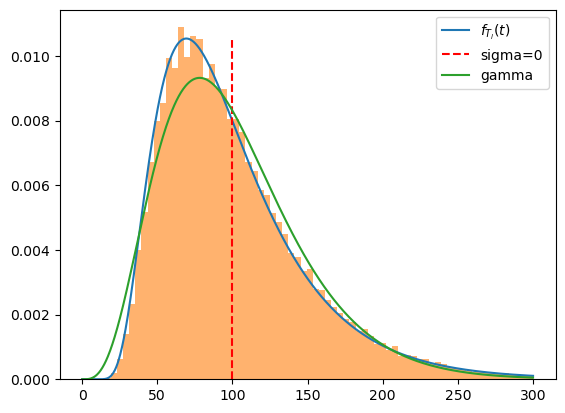
\includegraphics[width=\linewidth]{figures/Brownian motion w. drift distribution and montecarlo.png}
    \caption{Example of simulation and actual distribution. The marked $\sigma=0$ shows the limit as $\sigma \to 0$ corresponding to no noise on the input flow}
    \label{fig:1}
\end{figure}

\end{document}
